\documentclass [11pt, a4wide, twoside]{article}

\usepackage{times}
\usepackage{epsfig}
\usepackage{ifthen}
\usepackage{xspace}
\usepackage{fancyhdr}
\usepackage[colorlinks = true,linkcolor = black,urlcolor  = blue,citecolor = black,anchorcolor = black]{hyperref}
\usepackage{verbatim}
\usepackage{amsmath}
\usepackage{graphicx}

\usepackage{listings}
\usepackage{color}
%\usepackage{enumitem}

\definecolor{dkgreen}{rgb}{0,0.6,0}
\definecolor{gray}{rgb}{0.5,0.5,0.5}
\definecolor{mauve}{rgb}{0.58,0,0.82}

\lstset{frame=tb,
language=Java,
aboveskip=3mm,
belowskip=3mm,
showstringspaces=false,
columns=flexible,
basicstyle={\small\ttfamily},
numbers=none,
numberstyle=\tiny\color{gray},
keywordstyle=\color{blue},
commentstyle=\color{dkgreen},
stringstyle=\color{mauve},
breaklines=true,
breakatwhitespace=true
tabsize=3
}

\newboolean{showsolution}
\setboolean{showsolution}{true} 

% \newlist{todolist}{itemize}{2}
% \setlist[todolist]{label=$\square$}
% \usepackage{pifont}
% \newcommand{\cmark}{\ding{51}}%
% \newcommand{\xmark}{\ding{55}}%
% \newcommand{\done}{\rlap{$\square$}{\raisebox{2pt}{\large\hspace{1pt}\cmark}}%
% \hspace{-2.5pt}}
% \newcommand{\wontfix}{\rlap{$\square$}{\large\hspace{1pt}\xmark}}


% \usepackage{times}
\usepackage{epsfig}
\usepackage{ifthen}
\usepackage{xspace}
\usepackage{fancyhdr}
\usepackage{amsthm}
\usepackage{hyperref}



%layout
\topmargin      -5.0mm
\oddsidemargin  6.0mm
\evensidemargin -6.0mm
\textheight     215.5mm
\textwidth      160.0mm
\parindent      1.0em
\headsep        10.3mm
\headheight     12pt
\lineskip       1pt
\normallineskip 1pt

\newtheorem{mydef}{Definition}


%header
\lhead{Software Modeling and Analysis \\ 2016}

\rhead{Prof. Oscar Nierstrasz, Mohammad Ghafari, Nevena Milojkovi\'{c} and Yuriy Tymchuk}

\lfoot{page \thepage}
\rfoot{\today}
\cfoot{}

\renewcommand{\headrulewidth}{0.1pt}
\renewcommand{\footrulewidth}{0.1pt}

%enumeration
\newenvironment{myitemize}{%
     \begin{itemize}
     \setlength{\itemsep}{0cm}}
     {\end{itemize}}

\newenvironment{myenumerate}{%
     \begin{enumerate} \setlength{\itemsep}{0cm}}
     {\end{enumerate}}


%solution
\ifthenelse{\boolean{showsolution}}
   {  \newcommand{\solution}[1]{
   	\noindent\underline{\textbf{Answer:}}\\[2mm]
   	 \textsl{#1}
	 \vspace{10pt}
	 \normalsize
	}
  }
  {  \newcommand{\solution}[1]{} }


\pagestyle{fancy}

% ============================================================
% Markup macros for proof-reading
\usepackage{ifthen}
\usepackage[normalem]{ulem} % for \sout
\usepackage{xcolor}
\newcommand{\ra}{$\rightarrow$}
\newboolean{showedits}
\setboolean{showedits}{true} % toggle to show or hide edits
\ifthenelse{\boolean{showedits}}
{
	\newcommand{\ugh}[1]{\textcolor{red}{\uwave{#1}}} % please rephrase
	\newcommand{\ins}[1]{\textcolor{blue}{\uline{#1}}} % please insert
	\newcommand{\del}[1]{\textcolor{red}{\sout{#1}}} % please delete
	\newcommand{\chg}[2]{\textcolor{red}{\sout{#1}}{\ra}\textcolor{blue}{\uline{#2}}} % please change
}{
	\newcommand{\ugh}[1]{#1} % please rephrase
	\newcommand{\ins}[1]{#1} % please insert
	\newcommand{\del}[1]{} % please delete
	\newcommand{\chg}[2]{#2}
}
% ============================================================
% Put edit comments in a really ugly standout display
%\usepackage{ifthen}
\usepackage{amssymb}
\newboolean{showcomments}
\setboolean{showcomments}{true}
%\setboolean{showcomments}{false}
\newcommand{\id}[1]{$-$Id: scgPaper.tex 32478 2010-04-29 09:11:32Z oscar $-$}
\newcommand{\yellowbox}[1]{\fcolorbox{gray}{yellow}{\bfseries\sffamily\scriptsize#1}}
\newcommand{\triangles}[1]{{\sf\small$\blacktriangleright$\textit{#1}$\blacktriangleleft$}}
\ifthenelse{\boolean{showcomments}}
%{\newcommand{\nb}[2]{{\yellowbox{#1}\triangles{#2}}}
{\newcommand{\nbc}[3]{
 {\colorbox{#3}{\bfseries\sffamily\scriptsize\textcolor{white}{#1}}}
 {\textcolor{#3}{\sf\small$\blacktriangleright$\textit{#2}$\blacktriangleleft$}}}
 \newcommand{\version}{\emph{\scriptsize\id}}}
{\newcommand{\nbc}[3]{}
 \renewcommand{\ugh}[1]{#1} % please rephrase
 \renewcommand{\ins}[1]{#1} % please insert
 \renewcommand{\del}[1]{} % please delete
 \renewcommand{\chg}[2]{#2} % please change
 \newcommand{\version}{}}
\newcommand{\nb}[2]{\nbc{#1}{#2}{orange}}
\newcommand{\here}{\yellowbox{$\Rightarrow$ CONTINUE HERE $\Leftarrow$}}
\newcommand\rev[2]{\nb{TODO (rev #1)}{#2}} % reviewer comments
\newcommand\fix[1]{\nb{FIX}{#1}}
\newcommand\todo[1]{\nb{TO DO}{#1}}
\newcommand\on[1]{\nbc{ON}{#1}{red}} % add more author macros here
%\newcommand\XXX[1]{\nbc{XXX}{#1}{blue}}
%\newcommand\XXX[1]{\nbc{XXX}{#1}{brown}}
%\newcommand\XXX[1]{\nbc{XXX}{#1}{cyan}}
%\newcommand\XXX[1]{\nbc{XXX}{#1}{darkgray}}
%\newcommand\XXX[1]{\nbc{XXX}{#1}{gray}}
%\newcommand\XXX[1]{\nbc{XXX}{#1}{magenta}}
%\newcommand\XXX[1]{\nbc{XXX}{#1}{olive}}
%\newcommand\XXX[1]{\nbc{XXX}{#1}{orange}}
%\newcommand\XXX[1]{\nbc{XXX}{#1}{purple}}
%\newcommand\XXX[1]{\nbc{XXX}{#1}{red}}
%\newcommand\XXX[1]{\nbc{XXX}{#1}{teal}}
%\newcommand\XXX[1]{\nbc{XXX}{#1}{violet}}
%=============================================================
% ST80 listings macros
% Adapted from Squeak by Example book
%=============================================================
% If you want >>> appearing as right guillemet, you need these two lines:
%\usepackage[T1]{fontenc}
%\newcommand{\sep}{\mbox{>>}}
% Otherwise use this:
\newcommand{\sep}{\mbox{$\gg$}}
%=============================================================
%:\needlines{N} before code block to force page feed
\usepackage{needspace}
\newcommand{\needlines}[1]{\Needspace{#1\baselineskip}}
%=============================================================
%:Listings package configuration for ST80
\usepackage[english]{babel}
\usepackage{amssymb,textcomp}
\usepackage{listings}
% \usepackage[usenames,dvipsnames]{color}
% \usepackage[usenames]{color}
% \definecolor{source}{gray}{0.95}
\lstdefinelanguage{Smalltalk}{
%  morekeywords={self,super,true,false,nil,thisContext}, % This is overkill
  morestring=[d]',
  morecomment=[s]{"}{"},
  alsoletter={\#:},
  escapechar={!},
  literate=
    {BANG}{!}1
    {UNDERSCORE}{\_}1
    {\\st}{Smalltalk}9 % convenience -- in case \st occurs in code
    % {'}{{\textquotesingle}}1 % replaced by upquote=true in \lstset
    {_}{{$\leftarrow$}}1
    {>>>}{{\sep}}1
    {^}{{$\uparrow$}}1
    {~}{{$\sim$}}1
    {-}{{\sf -\hspace{-0.13em}-}}1  % the goal is to make - the same width as +
    {+}{\raisebox{0.08ex}{+}}1		% and to raise + off the baseline to match -
    {-->}{{\quad$\longrightarrow$\quad}}3
	, % Don't forget the comma at the end!
  tabsize=4
}[keywords,comments,strings]

\definecolor{source}{gray}{0.95}

\lstset{language=Smalltalk,
	basicstyle=\sffamily,
	keywordstyle=\color{black}\bfseries,
	% stringstyle=\ttfamily, % Ugly! do we really want this? -- on
	mathescape=true,
	showstringspaces=false,
	keepspaces=true,
	breaklines=true,
	breakautoindent=true,
	backgroundcolor=\color{source},
	lineskip={-1pt}, % Ugly hack
	upquote=true, % straight quote; requires textcomp package
	columns=fullflexible} % no fixed width fonts
% In-line code (literal)
% Normally use this for all in-line code:
\newcommand{\ct}{\lstinline[mathescape=false,backgroundcolor=\color{white},basicstyle={\sffamily\upshape}]}
% In-line code (latex enabled)
% Use this only in special situations where \ct does not work
% (within section headings ...):
\newcommand{\lct}[1]{{\textsf{\textup{#1}}}}
% Code environments
\lstnewenvironment{code}{%
	\lstset{%
		% frame=lines,
		frame=single,
		framerule=0pt,
		mathescape=false
	}
}{}

% Useful to add a matching $ after code containing a $
% \def\ignoredollar#1{}
%=============================================================
\newcommand{\ie}{\emph{i.e.}\xspace}
\newcommand{\eg}{\emph{e.g.}\xspace}
\newcommand{\etal}{\emph{et al.}\xspace}
% ============================================================

% \definecolor{mircolor}{rgb}{0.4,0.6,0.2}
% \newcommand\ml[1]{\nbc{ML}{#1}{mircolor}}
% \usepackage{wasysym}
% \newcommand\yesml[1]{\nbc{ML {\textcolor{yellow}\sun}}{#1}{mircolor}}

\usepackage{times}
\usepackage{epsfig}
\usepackage{ifthen}
\usepackage{xspace}
\usepackage{fancyhdr}
\usepackage{amsthm}
\usepackage{hyperref}



%layout
\topmargin      -5.0mm
\oddsidemargin  6.0mm
\evensidemargin -6.0mm
\textheight     215.5mm
\textwidth      160.0mm
\parindent      1.0em
\headsep        10.3mm
\headheight     12pt
\lineskip       1pt
\normallineskip 1pt

\newtheorem{mydef}{Definition}


%header
\lhead{Software Modeling and Analysis \\ 2016}

\rhead{Prof. Oscar Nierstrasz, Mohammad Ghafari, Nevena Milojkovi\'{c} and Yuriy Tymchuk}

\lfoot{page \thepage}
\rfoot{\today}
\cfoot{}

\renewcommand{\headrulewidth}{0.1pt}
\renewcommand{\footrulewidth}{0.1pt}

%enumeration
\newenvironment{myitemize}{%
     \begin{itemize}
     \setlength{\itemsep}{0cm}}
     {\end{itemize}}

\newenvironment{myenumerate}{%
     \begin{enumerate} \setlength{\itemsep}{0cm}}
     {\end{enumerate}}


%solution
\ifthenelse{\boolean{showsolution}}
   {  \newcommand{\solution}[1]{
   	\noindent\underline{\textbf{Answer:}}\\[2mm]
   	 \textsl{#1}
	 \vspace{10pt}
	 \normalsize
	}
  }
  {  \newcommand{\solution}[1]{} }


\pagestyle{fancy}

% ============================================================
% Markup macros for proof-reading
\usepackage{ifthen}
\usepackage[normalem]{ulem} % for \sout
\usepackage{xcolor}
\newcommand{\ra}{$\rightarrow$}
\newboolean{showedits}
\setboolean{showedits}{true} % toggle to show or hide edits
\ifthenelse{\boolean{showedits}}
{
	\newcommand{\ugh}[1]{\textcolor{red}{\uwave{#1}}} % please rephrase
	\newcommand{\ins}[1]{\textcolor{blue}{\uline{#1}}} % please insert
	\newcommand{\del}[1]{\textcolor{red}{\sout{#1}}} % please delete
	\newcommand{\chg}[2]{\textcolor{red}{\sout{#1}}{\ra}\textcolor{blue}{\uline{#2}}} % please change
}{
	\newcommand{\ugh}[1]{#1} % please rephrase
	\newcommand{\ins}[1]{#1} % please insert
	\newcommand{\del}[1]{} % please delete
	\newcommand{\chg}[2]{#2}
}
% ============================================================
% Put edit comments in a really ugly standout display
%\usepackage{ifthen}
\usepackage{amssymb}
\newboolean{showcomments}
\setboolean{showcomments}{true}
%\setboolean{showcomments}{false}
\newcommand{\id}[1]{$-$Id: scgPaper.tex 32478 2010-04-29 09:11:32Z oscar $-$}
\newcommand{\yellowbox}[1]{\fcolorbox{gray}{yellow}{\bfseries\sffamily\scriptsize#1}}
\newcommand{\triangles}[1]{{\sf\small$\blacktriangleright$\textit{#1}$\blacktriangleleft$}}
\ifthenelse{\boolean{showcomments}}
%{\newcommand{\nb}[2]{{\yellowbox{#1}\triangles{#2}}}
{\newcommand{\nbc}[3]{
 {\colorbox{#3}{\bfseries\sffamily\scriptsize\textcolor{white}{#1}}}
 {\textcolor{#3}{\sf\small$\blacktriangleright$\textit{#2}$\blacktriangleleft$}}}
 \newcommand{\version}{\emph{\scriptsize\id}}}
{\newcommand{\nbc}[3]{}
 \renewcommand{\ugh}[1]{#1} % please rephrase
 \renewcommand{\ins}[1]{#1} % please insert
 \renewcommand{\del}[1]{} % please delete
 \renewcommand{\chg}[2]{#2} % please change
 \newcommand{\version}{}}
\newcommand{\nb}[2]{\nbc{#1}{#2}{orange}}
\newcommand{\here}{\yellowbox{$\Rightarrow$ CONTINUE HERE $\Leftarrow$}}
\newcommand\rev[2]{\nb{TODO (rev #1)}{#2}} % reviewer comments
\newcommand\fix[1]{\nb{FIX}{#1}}
\newcommand\todo[1]{\nb{TO DO}{#1}}
\newcommand\on[1]{\nbc{ON}{#1}{red}} % add more author macros here
%\newcommand\XXX[1]{\nbc{XXX}{#1}{blue}}
%\newcommand\XXX[1]{\nbc{XXX}{#1}{brown}}
%\newcommand\XXX[1]{\nbc{XXX}{#1}{cyan}}
%\newcommand\XXX[1]{\nbc{XXX}{#1}{darkgray}}
%\newcommand\XXX[1]{\nbc{XXX}{#1}{gray}}
%\newcommand\XXX[1]{\nbc{XXX}{#1}{magenta}}
%\newcommand\XXX[1]{\nbc{XXX}{#1}{olive}}
%\newcommand\XXX[1]{\nbc{XXX}{#1}{orange}}
%\newcommand\XXX[1]{\nbc{XXX}{#1}{purple}}
%\newcommand\XXX[1]{\nbc{XXX}{#1}{red}}
%\newcommand\XXX[1]{\nbc{XXX}{#1}{teal}}
%\newcommand\XXX[1]{\nbc{XXX}{#1}{violet}}
%=============================================================
% ST80 listings macros
% Adapted from Squeak by Example book
%=============================================================
% If you want >>> appearing as right guillemet, you need these two lines:
%\usepackage[T1]{fontenc}
%\newcommand{\sep}{\mbox{>>}}
% Otherwise use this:
\newcommand{\sep}{\mbox{$\gg$}}
%=============================================================
%:\needlines{N} before code block to force page feed
\usepackage{needspace}
\newcommand{\needlines}[1]{\Needspace{#1\baselineskip}}
%=============================================================
%:Listings package configuration for ST80
\usepackage[english]{babel}
\usepackage{amssymb,textcomp}
\usepackage{listings}
% \usepackage[usenames,dvipsnames]{color}
% \usepackage[usenames]{color}
% \definecolor{source}{gray}{0.95}
\lstdefinelanguage{Smalltalk}{
%  morekeywords={self,super,true,false,nil,thisContext}, % This is overkill
  morestring=[d]',
  morecomment=[s]{"}{"},
  alsoletter={\#:},
  escapechar={!},
  literate=
    {BANG}{!}1
    {UNDERSCORE}{\_}1
    {\\st}{Smalltalk}9 % convenience -- in case \st occurs in code
    % {'}{{\textquotesingle}}1 % replaced by upquote=true in \lstset
    {_}{{$\leftarrow$}}1
    {>>>}{{\sep}}1
    {^}{{$\uparrow$}}1
    {~}{{$\sim$}}1
    {-}{{\sf -\hspace{-0.13em}-}}1  % the goal is to make - the same width as +
    {+}{\raisebox{0.08ex}{+}}1		% and to raise + off the baseline to match -
    {-->}{{\quad$\longrightarrow$\quad}}3
	, % Don't forget the comma at the end!
  tabsize=4
}[keywords,comments,strings]

\definecolor{source}{gray}{0.95}

\lstset{language=Smalltalk,
	basicstyle=\sffamily,
	keywordstyle=\color{black}\bfseries,
	% stringstyle=\ttfamily, % Ugly! do we really want this? -- on
	mathescape=true,
	showstringspaces=false,
	keepspaces=true,
	breaklines=true,
	breakautoindent=true,
	backgroundcolor=\color{source},
	lineskip={-1pt}, % Ugly hack
	upquote=true, % straight quote; requires textcomp package
	columns=fullflexible} % no fixed width fonts
% In-line code (literal)
% Normally use this for all in-line code:
\newcommand{\ct}{\lstinline[mathescape=false,backgroundcolor=\color{white},basicstyle={\sffamily\upshape}]}
% In-line code (latex enabled)
% Use this only in special situations where \ct does not work
% (within section headings ...):
\newcommand{\lct}[1]{{\textsf{\textup{#1}}}}
% Code environments
\lstnewenvironment{code}{%
	\lstset{%
		% frame=lines,
		frame=single,
		framerule=0pt,
		mathescape=false
	}
}{}

% Useful to add a matching $ after code containing a $
% \def\ignoredollar#1{}
%=============================================================
\newcommand{\ie}{\emph{i.e.}\xspace}
\newcommand{\eg}{\emph{e.g.}\xspace}
\newcommand{\etal}{\emph{et al.}\xspace}
% ============================================================


\begin{document}

\section*{\ifthenelse{\boolean{showsolution}}{\textcolor{red}{Solution}\\}{}Assignment 09 --- 11.11.2020 -- v1.2\\Static Program Analysis}

\textcolor{red}{Please submit this exercise by email to \href{mailto:pascal.gadient@inf.unibe.ch}{pascal.gadient@inf.unibe.ch} \underline{before} 18 November 2020, 10:15am.\begin{center}\textbf{You must submit your code as editable text, i.e., use plain text file(s).}\end{center}}

\noindent For the second part of this exercise, we use the latest GT release from \href{https://gtoolkit.com/download/}{here}. If you already imported some Moose (MSE) models from the previous assignments into your GT environment, please start with a fresh copy of GT to reduce the strains on your computer's random access memory.
\\\\
\noindent First, we have to download and extract the \emph{Weka} dataset, and second, we need to import it into GT. We can perform both tasks using GT's Playground. Be warned: this process will take several minutes depending on your device's CPU and internet connection. We strongly advise you to save the image when the process succeeded to avoid redoing these steps.\\

\noindent The datasets can be downloaded and extracted with the following script:\\\\
\texttt{targetFolder := (FileLocator imageDirectory asFileReference / \textquotesingle models\textquotesingle) ensureCreateDirectory.\\
archiveFileName := \textquotesingle weka-3-8.zip\textquotesingle.\\
archiveUrl := \textquotesingle https://dl.feenk.com/moose-tutorial/weka/\textquotesingle.\\
ZnClient new\\
\hspace*{0.5cm}url: archiveUrl, archiveFileName;\\
\hspace*{0.5cm}signalProgress: true;\\
\hspace*{0.5cm}downloadTo: targetFolder.\\
(ZipArchive new\\
\hspace*{0.5cm}readFrom: targetFolder / archiveFileName)\\
\hspace*{0.5cm}extractAllTo: targetFolder.}\\

\noindent The sample dataset can be imported with the following script:\\\\
\texttt{modelFile := (FileLocator imageDirectory asFileReference / \textquotesingle models\textquotesingle)\\
\hspace*{0.5cm}/ \textquotesingle weka-3-8\textquotesingle\\
\hspace*{0.5cm}/ \textquotesingle weka-3-8.mse\textquotesingle.\\
modelWeka := MooseModel new\\
\hspace*{0.5cm}importMSEFromFile: modelFile.}

\newpage

\subsection*{Exercise 1: Theory (3.5 pts)}
\begin{enumerate}[a)]
\item What is the difference between static and dynamic code analysis?
\solution{Static code analysis is performed without executing any code but only observing source code, whereas dynamic code analysis is performed during the execution of code observing the current state of the application. Both analyses have individual advantages and limitations. For example, static analyses nicely scale vertically (by increasing the CPU speed or count) or horizontally (by adding more devices to the analysis infrastructure), and they can produce accurate results. However, they usually do not consider the executing environment (app configuration, build system, etc.) and the results might not be very comprehensive and suffer from many false positives or false negatives. On the other hand, dynamic analyses are harder to scale, because each analysis needs its own execution environment. On the bright side, they enable analyses that work on any executable code; even code that became available with the execution of the application, \eg software updates.}
\item Suppose you want to analyze the code that a method downloads arbitrarily from the internet. Can you perform such an inspection with \emph{static analyses}? If yes, how, if not, why not?
\solution{No, because you cannot inspect code fetched at run time with static analysis tools. To circumvent this problem, analysts usually extract the corresponding URL statically and then download and manually analyze that code.}
\item Suppose you want to analyze the code that a method downloads arbitrarily from the internet. Can you perform such an inspection with \emph{dynamic analyses}? If yes, how, if not, why not?
\solution{Yes, because a dynamic analysis involves the execution of arbitrary code. When the code is under test, it will be executed in the analysis environment and thus download and also execute the requested code.}
\item Choose a static analysis scenario where it is crucial to have no type 1 errors (false positives), but type 2 errors (false negatives) can be accepted. Explain for your scenario why you can accept type 2 errors, but no type 1 errors.
\solution{Dead code elimination. If such a tool suffers from false positives (dead code that isn't actually dead) it would cause serious problems as soon as it tries to remove affected code, because the code is still in use. On the contrary, false negatives are less harmful, because they only avoid that orphaned code is removed which does not break the system.}
\item Choose a statically-typed language, and briefly describe what makes it statically-typed.
\solution{In statically-typed languages, types are assigned to variables at compile-time. Such languages provide the benefits of having a static type system at various places, \eg in the IDE with live feedback about potential mistakes and improvements, or in Unit testing frameworks. \emph{Java:} The type of each variable must be declared explicitly in the source code. There exist generic types that can represent different types during run time, but Java still validates generic types at compile-time. Generically-typed variables cannot change their type once they have been initialized.}
\item Choose a dynamically-typed language, and briefly describe what makes it dynamically-typed.
\solution{In dynamically-typed languages, types are assigned to variables at run time and in many languages they can even change depending on the assigned values. Code in such languages does not need to hold any type information and is more compact (improves readability and efficiency of developers), however the dynamic nature of the execution usually impacts performance and leads to more subtile bugs during execution time, \eg code does work but not as expected. \emph{Smalltalk:} The source code does not need any type information. Instead, types that do not match result in a \texttt{doesNotUnderstand} message.}
\item Is the collection of variable name declarations in the method body of Java's \\\texttt{PrintStream.println(String s)} intraprocedural or interprocedural? Explain why.
\solution{The scope of intraprocedural analyses remains within a particular method (\eg searching for \texttt{if} statements within a method), whereas the scope of interprocedural analyses could include the whole project (\eg tracking of variable values through different classes and methods). The collection of variable name declarations in a method is an intraprocedural analysis, because it only requires look ups for entities within a particular method. The look up could be performed by traversing the AST of the method while collecting all \texttt{Variable\-Declar\-ation} nodes.}
\end{enumerate}

\newpage

\subsection*{Exercise 2: Control flow graphs (6.5 pts)}
\begin{enumerate}[a)]
\item Draw a CFG by hand (or with a flow chart tool) for the following code block: (1.5 pts)\\
\texttt{int a = 2;\\
int b = 3;\\
if (a == 2) \{\\
\hspace*{0.5cm}b = a + b;\\
\} else \{\\
\hspace*{0.5cm}b = a++;\\
\}\\
return a + b;}\\
\solution{\begin{figure}[h]
\centering
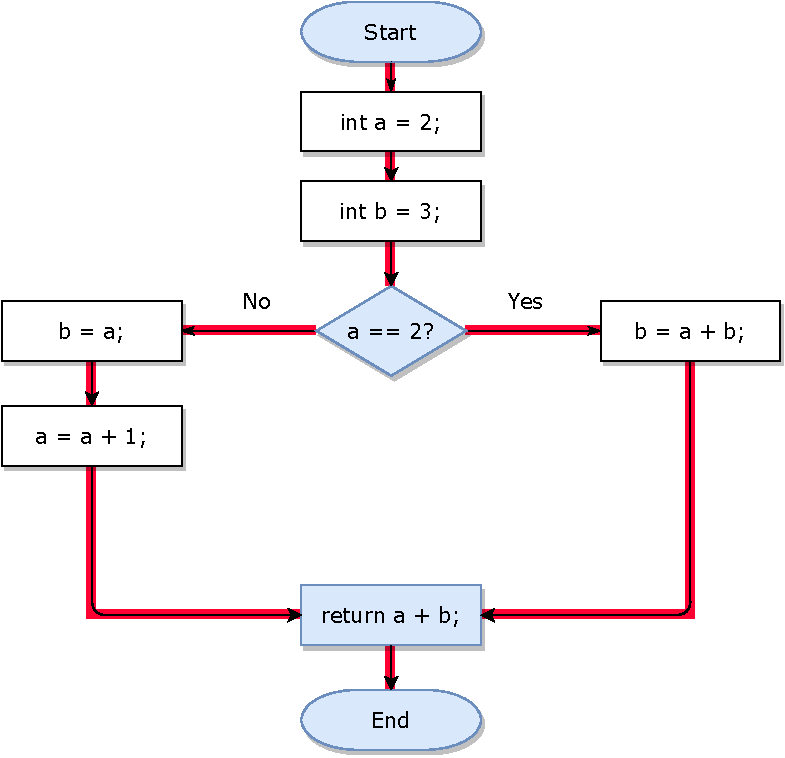
\includegraphics[scale=0.6]{figures/2a.pdf}
\end{figure}}
\ifthenelse{\boolean{showsolution}}{\newpage}{}
\item Draw a CFG by hand (or with a flow chart tool) for the following code block: (2 pts)\\
\texttt{public boolean addBalances(int money) \{\\
\hspace*{0.5cm}if (money \textgreater~0) \{\\
\hspace*{1.0cm}acquire(lock);\\
\hspace*{1.0cm}int newMoneyValue = this.money + money;\\
\hspace*{1.0cm}if (newMoneyValue \textless~MAX\_MONEY) \{\\
\hspace*{1.5cm}this.money = newMoneyValue;\\
\hspace*{1.5cm}release(lock);\\
\hspace*{1.5cm}return true;\\
\hspace*{1.0cm}\} else \{\\
\hspace*{1.5cm}release(lock);\\
\hspace*{1.5cm}return false;\\
\hspace*{1.0cm}\}\\
\hspace*{0.5cm}\} else \{\\
\hspace*{1.0cm}return false;\\
\hspace*{0.5cm}\}\\
\}\\}
\solution{\begin{figure}[h]
\centering
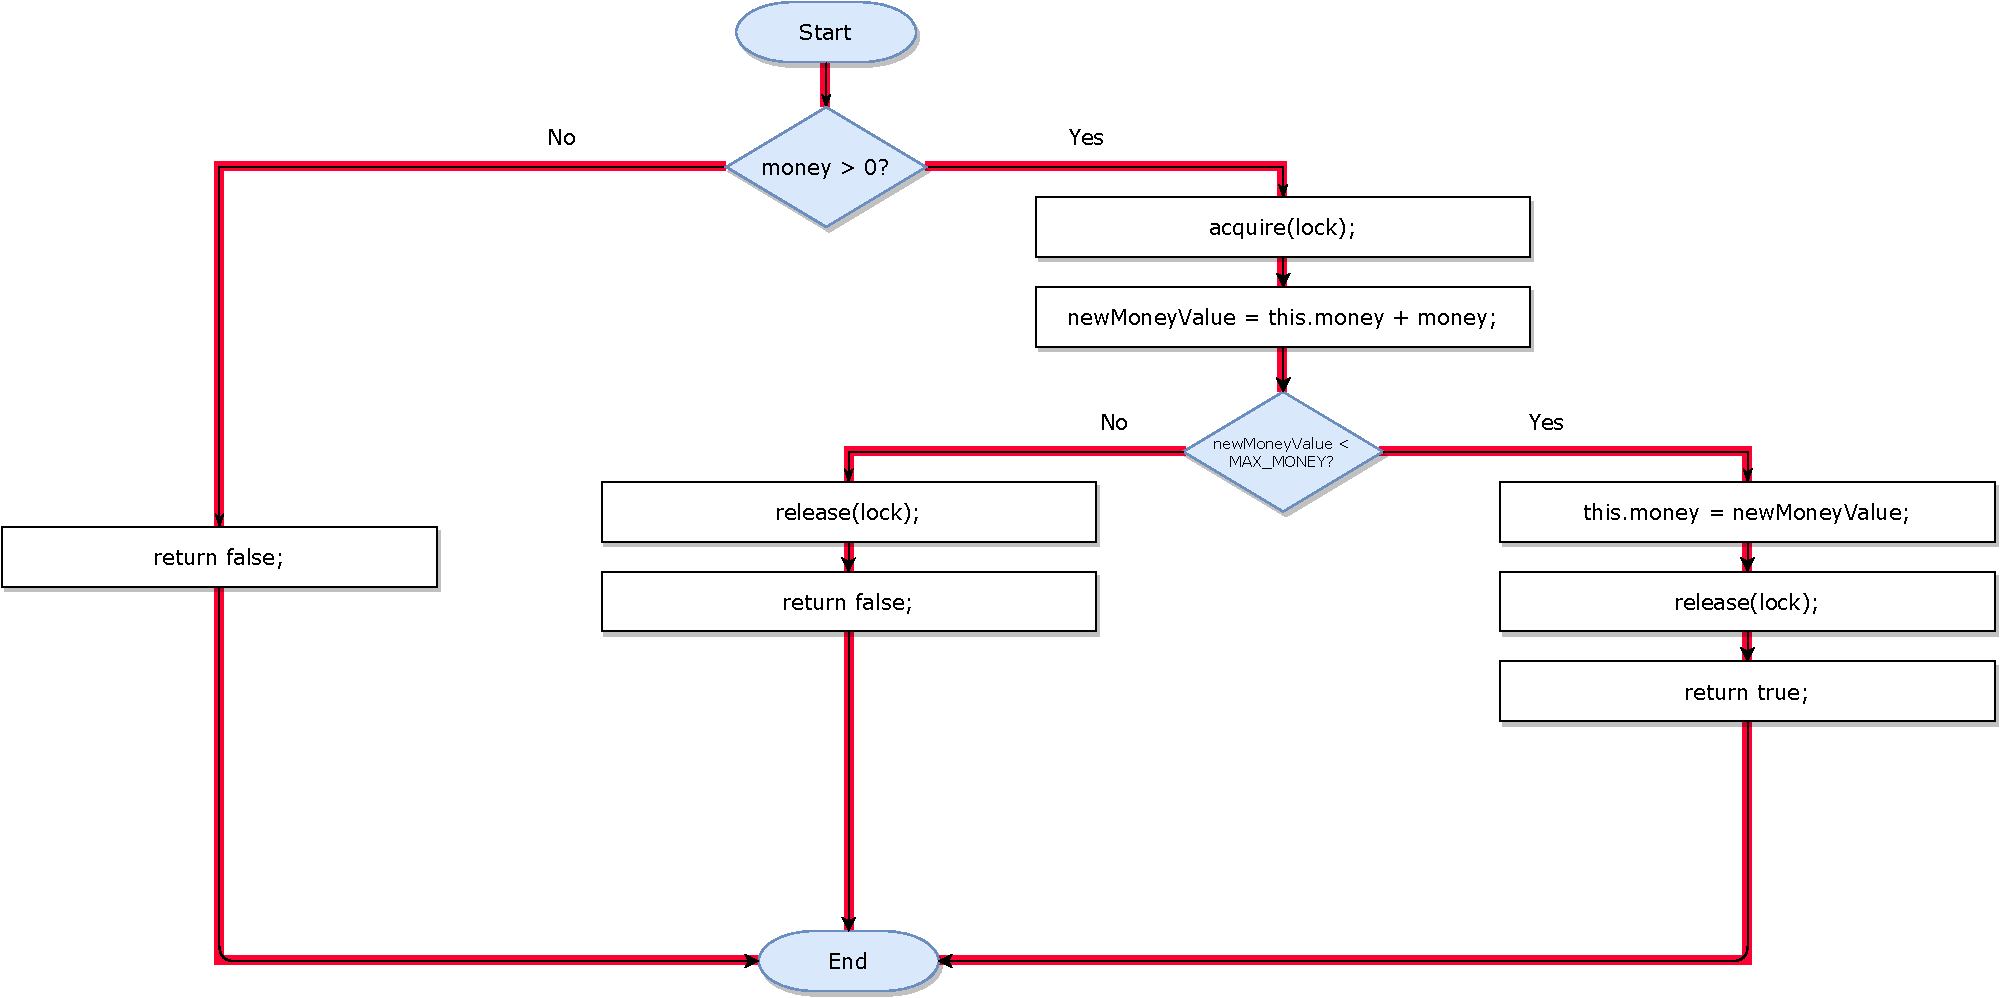
\includegraphics[scale=0.4]{figures/2b.pdf}
\end{figure}
\ifthenelse{\boolean{showsolution}}{\newpage}{}}
\item What is the cyclomatic complexity of both code blocks, i.e., from task a) and task b)? You should use the formula from A08. (1 pt)
\solution{The cyclomatic complexity can be calculated with the following formula: M = E - N + 2. In the previous CFGs we colored the edges in red, and the relevant nodes in light blue. The (white) statement nodes do not contribute to the nodes required by the formula, \ie they are ``invisible'' for the cyclo computation. For a) the formula yields M = 4 - 4 + 2 = 2 and for b) it yields M = 5 - 4 + 2 = 3.}
\item Create the interval CFG for both code blocks, i.e., from task a) and task b). You can find an example CFG at the bottom of slide 20 (page 32) in the slide deck of lecture 09 which is available \href{http://scg.unibe.ch/download/lectures/sma/SMA-09-StaticAnalysis.pdf}{here}. (2 pts)
\solution{\begin{figure}[h]
\centering
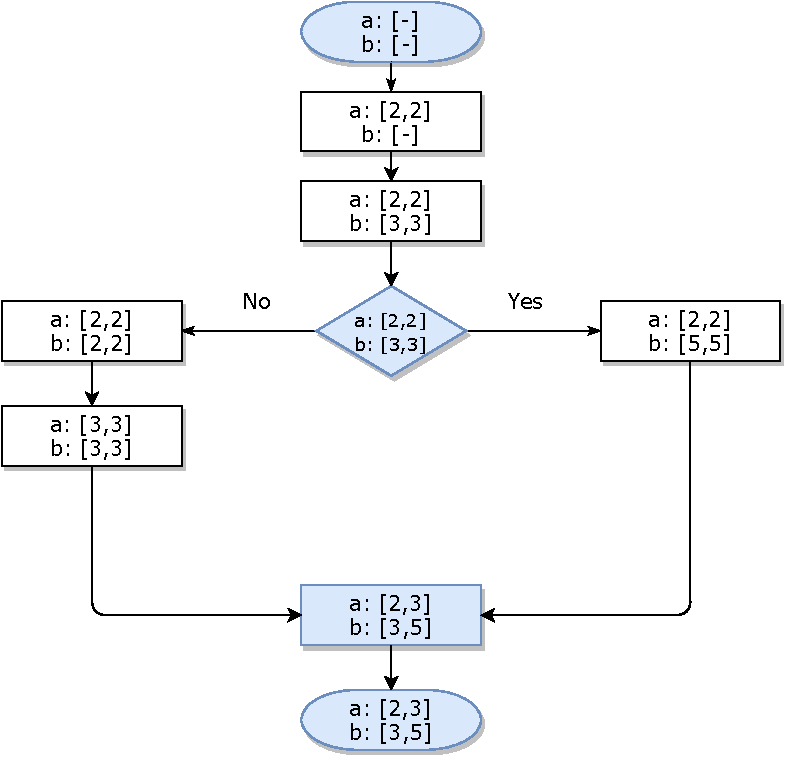
\includegraphics[scale=0.4]{figures/2d1.pdf}
\end{figure}
\begin{figure}[h]
\centering
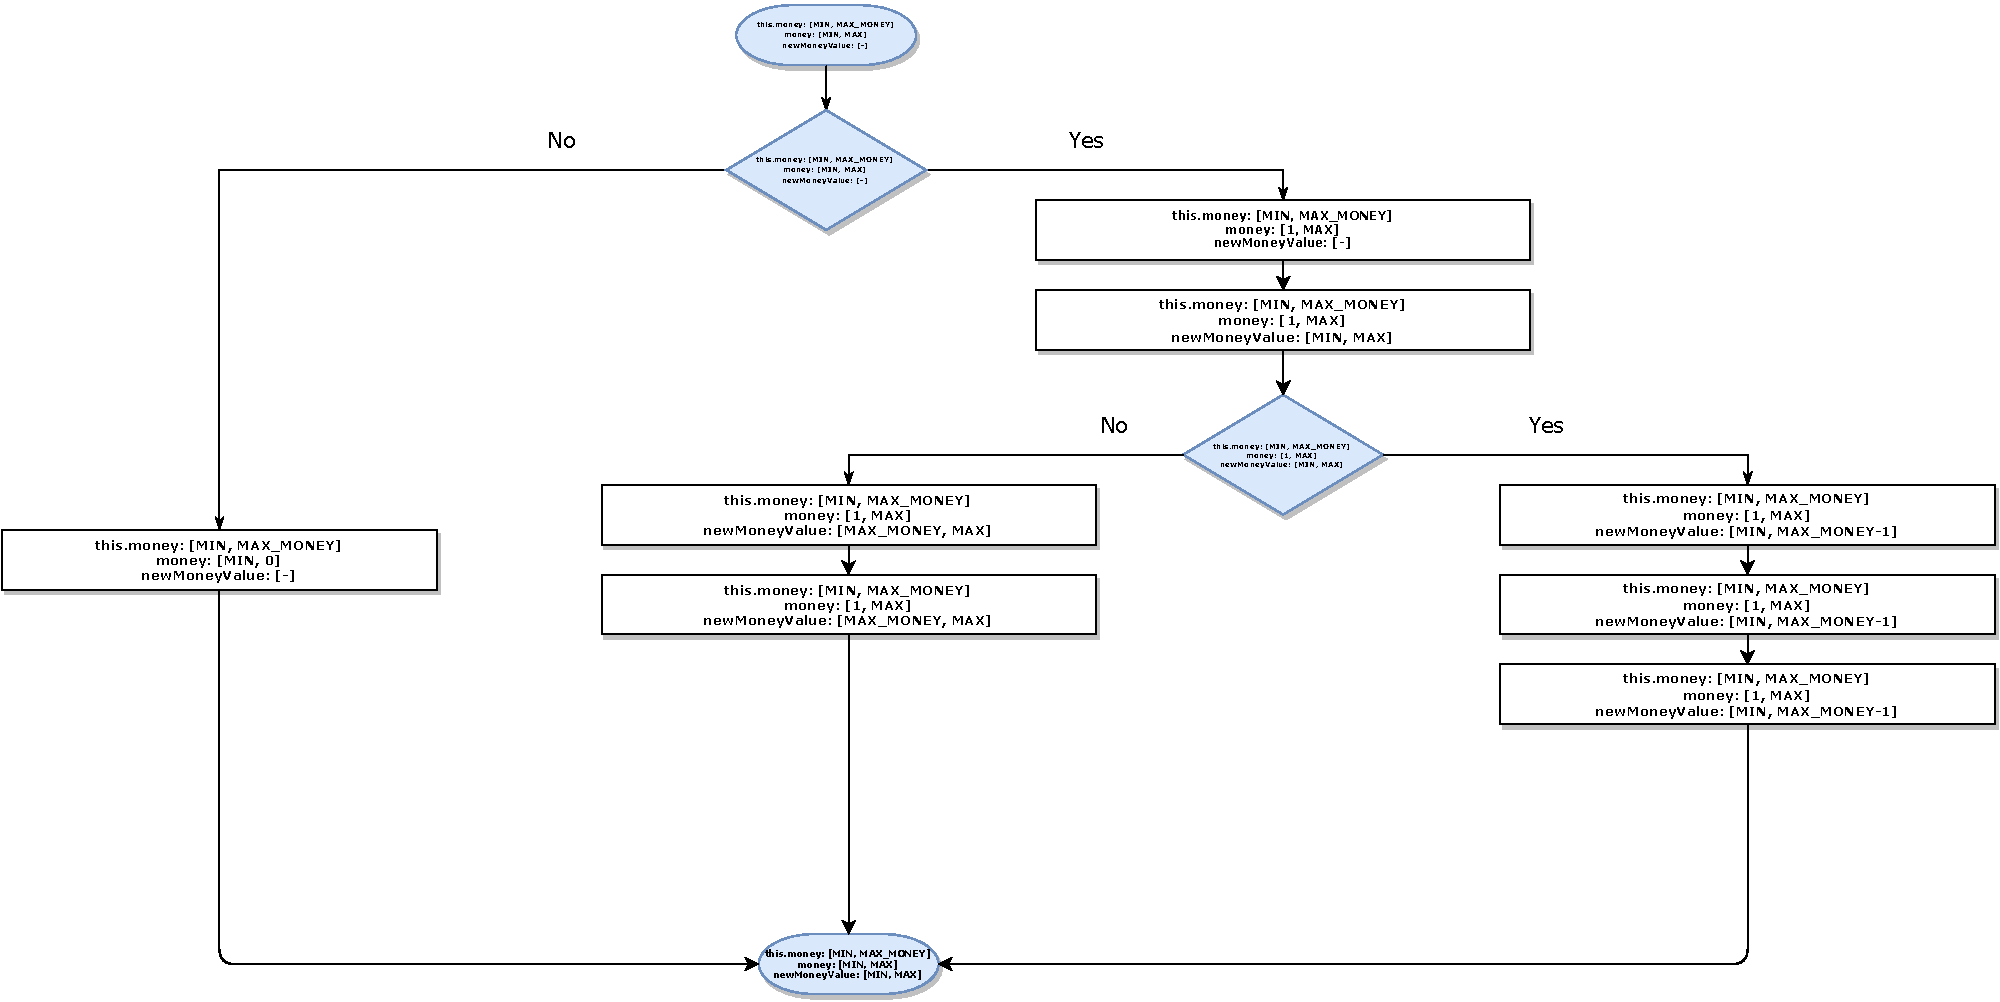
\includegraphics[scale=0.4]{figures/2d2.pdf}
\end{figure}}
\end{enumerate}

% \subsection*{Exercise 3: Recursive methods (3 pts BONUS)}
% Your task is to find and visualize all recursive methods in \texttt{modelWeka}.

% \solution{\texttt{
%     tests := modelWeka allModelMethods select: [ :each | each namespaceScope asString beginsWith: 'weka (Namespace)::associations (Namespace)'] .

%     eager := tests select: [ : m |
%         | asserts astNode |
%         asserts := OrderedCollection new.
%         astNode := m gtASTNode.
%         astNode
%             ifNotNil: [ astNode
%                     allNodesOfType: JavaMethodInvocationNode
%                     do: [ :node | 
%                         (node asString = m asString)
%                             ifTrue: [ asserts add: node ] ] ].
%         asserts size > 1 ].}}

\newpage

\subsection*{Exercise 3: Template methods (6 pts BONUS)}
Find all template methods in \texttt{modelWeka} with the help of \texttt{\#gtASTNode}s, and plot them with \texttt{GtMondrian}. Please follow the steps below, one after another. The resulting plot should look similar to~\autoref{fig:mondrian}.\\\\
\emph{NB: Template methods are abstract methods (in classes or interfaces).}\\\\
\emph{Step 1:}
Select all methods that are in the namespace scope \texttt{weka::core}.\\\\
\emph{Step 2:}
Of those methods, find those that are abstract. Use \texttt{gtASTNode} for the AST traversal. You can search for \texttt{JavaAbstractMethodDeclarationNode} nodes to find the relevant methods.\\\\
\emph{In this step, GT will build the AST of the relevant entities. This requires several minutes and around 6 GB of RAM on your PC. If you have less RAM the computation will slowdown massively. Note: There is currently a bug in the FAMIX implementation that avoids proper detection of abstract methods in classes.}\\\\
\emph{Step 3:}
Visualize the found methods in \emph{Step 2} with \texttt{GtMondrian}. Use the following parameters:
\begin{itemize}
\item shape type: \texttt{BlElement} with a size that represents \texttt{\#children} of each method
\item shape geometry: \texttt{BlCircle}
\item shape background: all methods that have more than three elements in \texttt{children} should be in red, the others in gray
\end{itemize}
\begin{figure}[h]
\centering
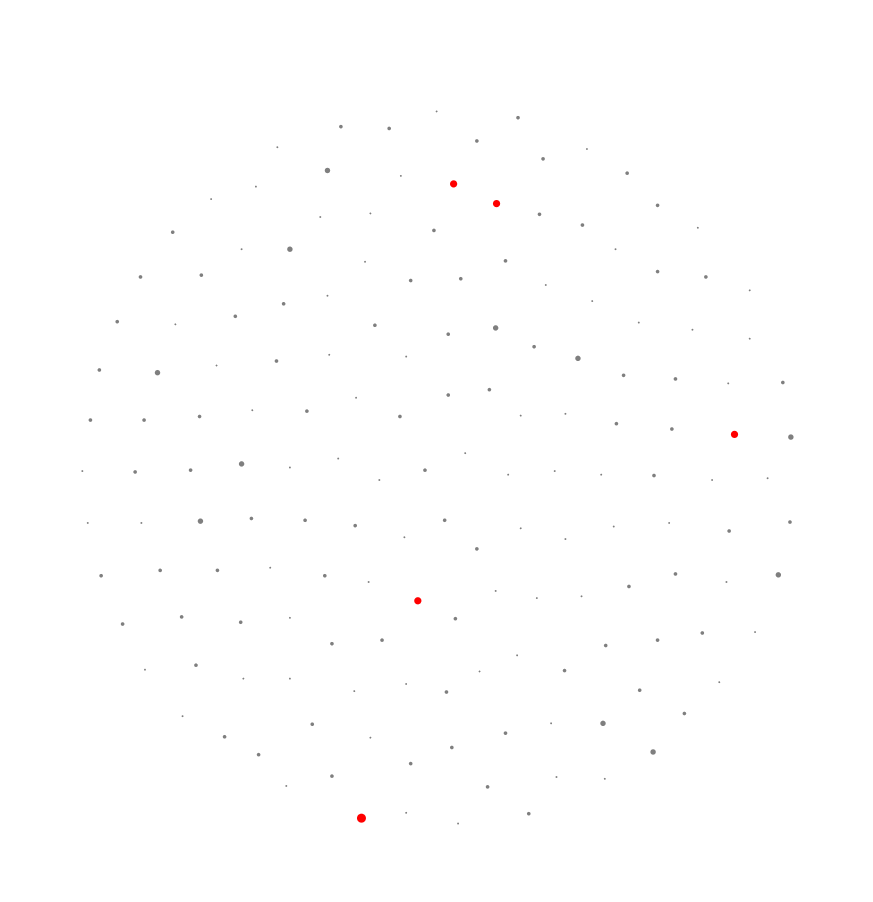
\includegraphics[scale=0.38]{figures/mondrian.png}
\caption{The resulting GtMondrian visualization built with GT}
\label{fig:mondrian}
\end{figure}
\solution{\texttt{
sampleClasses := modelWeka allModelMethods select: [ :each \textbar\\
\hspace*{0.5cm}each namespaceScope asString beginsWith:\\
\hspace*{1.0cm}\textquotesingle weka (Namespace)::core (Namespace)\textquotesingle].\\\\
templateMethods := sampleClasses select: [ :m \textbar\\
\textbar~templateMethod astNode \textbar\\
astNode := m gtASTNode.\\
astNode ifNotNil: [	\\
\hspace*{0.5cm}(astNode isMemberOf: JavaAbstractMethodDeclarationNode)\\
\hspace*{1.0cm}ifTrue: [  templateMethod := true. ] ].\\
templateMethod = true. ].\\\\
view := GtMondrian new.\\
view nodes\\
\hspace*{0.5cm}shape:  [ :m \textbar\\
\hspace*{1.0cm}BlElement new size:  m children size @ m children size;\\
\hspace*{1.0cm}geometry:  BlCircle new;\\
\hspace*{1.0cm}background:	((m children size \textgreater~3)\\
\hspace*{1.5cm}ifTrue: [ Color red ]\\
\hspace*{1.5cm}ifFalse: [ Color gray ])];\\
\hspace*{0.5cm}with:  templateMethods.\\
view layout force.\\
view.}}
% \subsection*{Exercise 4: Template methods (3 pts BONUS)}
% I thought some suitable exercises could be to write queries for some common patterns or anti-patterns such as template methods. (Find methods that invoke same class methods that are abstract.) I did not try it myself yet though. in \texttt{modelWeka}.

% \solution{\texttt{
% matches := OrderedCollection new.\\
% modelWeka allModelMethods do: [ :each \textbar\\
% ((each invokedMethods do: [ :outgoingCall \textbar~outgoingCall = each])\\
% size \textgreater~0)\\
% ifTrue: [ matches add: each. ] ]}}

% \subsection*{Exercise 2: Detection of unreachable root classes (4 pts)}
% Your task is to find and visualize all unreachable root classes in \texttt{modelWeka}. This task consists of four different steps, one after another.

% \begin{enumerate}[{Step} 1)]
% \item Find all methods reachable from main. You can use \texttt{invokedMethods} to find the initial invoked methods, and then you do have to repeat this process until you find no more invoked methods. (2 pts)
% \solution{\texttt{reachableMethods := Set new.\\
% methodsToCheck := (modelWeka allModelMethods select: \\
% \hspace*{0.5cm}[ :m \textbar~m name = \textquotesingle main\textquotesingle~]) entities.\\
% \hspace*{0.0cm}[ methodsToCheck notEmpty ] whileTrue: [ \textbar~m \textbar\\
% \hspace*{0.5cm}m := methodsToCheck removeFirst.\\
% \hspace*{0.5cm}m invokedMethods do: [ :each \textbar\\
% \hspace*{0.5cm}(reachableMethods includes: each) \\
% \hspace*{1.0cm}ifFalse: [  methodsToCheck add: each.\\
% \hspace*{1.5cm}reachableMethods add: each ] ] ].\\
% reachableMethods.}}
% \item Find the classes of reachable methods. (3 pts)
% \solution{\texttt{
% reachableClasses := reachableMethods collect: \#parentType.\\
% "Add classes accessed by reachable methods"\\
% reachableClasses addAll: ((((reachableMethods flatCollect: \#accesses) collect: \#variable) select: \#isAttribute) collect: \#parentType).\\
% "Add all superclasses and subclasses"\\
% reachableClasses addAll: (reachableClasses flatCollect: \\
% \hspace*{0.5cm}\#withSuperclassHierarchy).\\
% "Add all classes referenced from reachable methods"\\
% reachableClasses addAll: (reachableMethods flatCollect:\\
% \hspace*{0.5cm}\#providerTypes).\\
% "Recursively add all classes referenced from reachable classes"\\
% newTypes := reachableClasses flatCollect: \#allProviderTypes.\\
% newTypes removeAllFoundIn: reachableClasses.\\
% \hspace*{0.0cm}[ newTypes notEmpty ]\\
% \hspace*{0.5cm}whileTrue: [\\
% \hspace*{1.0cm}reachableClasses addAll: newTypes.\\
% \hspace*{1.0cm}newTypes := reachableClasses flatCollect: \#allProviderTypes.\\
% \hspace*{1.0cm}newTypes removeAllFoundIn: reachableClasses ].\\
% reachableClasses.}}
% \ifthenelse{\boolean{showsolution}}{\newpage}{}
% \item Find all unreachable classes from the main method. (1 pt BONUS)\\\\\emph{NB: Unreachable classes are the complement of the reachable ones.}
% \solution{\texttt{unReachableClasses := modelWeka allModelClasses copy.\\
% unReachableClasses removeAllFoundIn: reachableClasses.\\
% "Ignore inner classes"\\
% unReachableClasses removeAllSuchThat: \#isInnerClass.\\
% unReachableClasses.}}
% \item Create a \texttt{GtMondrian} visualization that shows the unreachable classes. Unreachable classes must be in red. Your plot should be similar to the one in~\autoref{fig:mondrian}. (2 pts BONUS)
% \solution{\texttt{view := GtMondrian new.\\
% view nodes\\
% \hspace*{0.5cm}shape: [ :m \textbar \\
% \hspace*{1.0cm}BlElement new\\
% \hspace*{1.5cm}size: 5@5;\\
% \hspace*{1.5cm}geometry: BlCircle new;\\
% \hspace*{1.5cm}background: ((m fanIn = 0)\\
% \hspace*{2.0cm}ifTrue: [ Color red ]\\
% \hspace*{2.0cm}ifFalse: [ Color gray ])];\\
% \hspace*{1.5cm}with: unReachableClasses.\\
% view edges connectFromAll: \#providerTypes.\\
% view layout force.\\
% view.}
% \begin{figure}[h]
% \centering
% 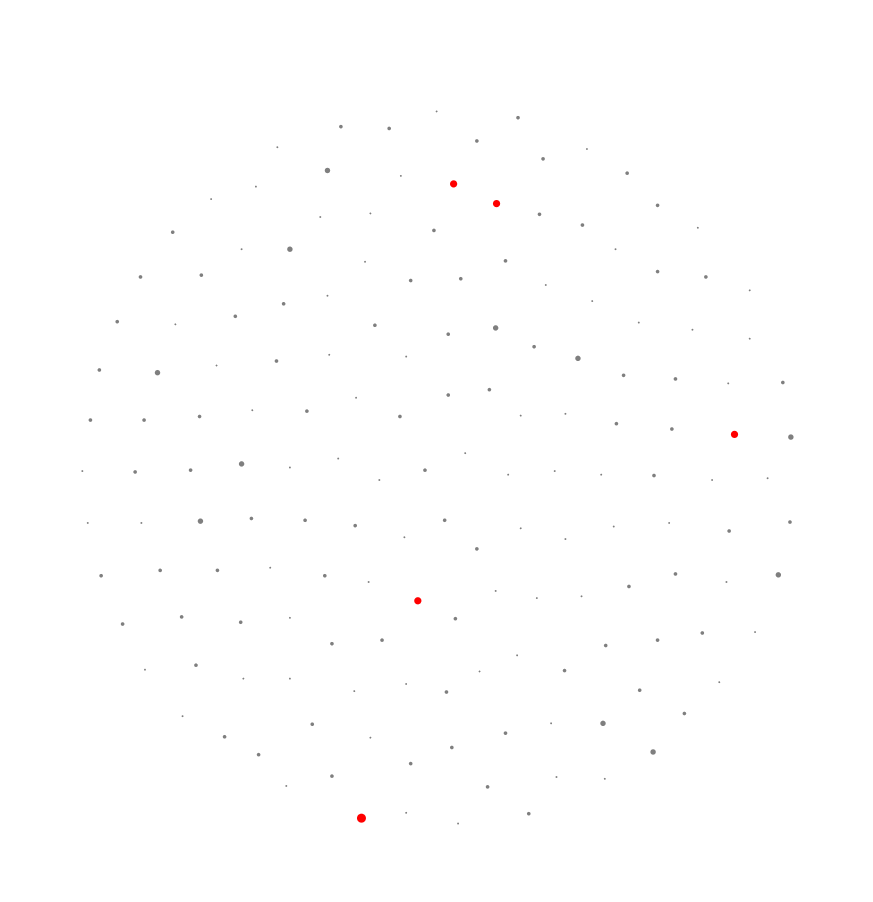
\includegraphics[scale=0.27]{figures/mondrian.png}
% \caption{The resulting GtMondrian visualization built with GT}
% \label{fig:mondrian}
% \end{figure}
% }
% \end{enumerate}

\end{document}
